\documentclass[12pt, a4paper]{article}
\usepackage[utf8]{inputenc}
\usepackage{indentfirst} %indentace prvního odstavce
\usepackage{mathtools}
\usepackage{amsfonts}
\usepackage{amsmath}
\usepackage{amssymb}
\usepackage{graphicx}
\usepackage[czech]{babel}
\DeclarePairedDelimiter{\ceil}{\lceil}{\rceil}

\begin{document}

\section{}
Označme si vybraný počet součástek vektorem $n=(n_{k_1},n_{k_2},n_{t_1},n_{t_2})^T$, kde $n_{k_1}$ odpovídá počtu normálních kondenzátorů, $n_{k_2}$ kvalitních kondenzátorů, $n_{t_1}$ normálních tranzistorů a $n_{t_2}$ kvalitních tranzistorů. Ze zadání víme, že součástka by měla vydržet cca 2.5 roku. Tudíž můžeme shora odhadnout maximální počet každé součastky, protože usoudíme, že součástka by neměla mít větší životnost než 3 roky. Obvod samotný vydrží 1 rok, takže po součástkách chceme dohromady maximálně 2 roky (24 měsíců).

Označme $A = (0.2,0.83,0.85,1.3)$ matici (vektor) \uv{životnosti} a $B = (0.1,1,0.35,0.5)$ matici (vektor) ceny. Jelikož přidaná životnost v měsích součástky sestavené dle vektoru $n$ se spočítá $A \cdot n$ a cena $B \cdot n$.

Maximální počet pro každou součástku je postupně dle značení výše $m_{k_1}=\ceil{\frac{24}{0.2}}=120, \ m_{k_2}=\ceil{\frac{24}{0.83}}=29, \ m_{t_1}=\ceil{\frac{24}{0.85}}=29,\ m_{t_2}=\ceil{\frac{24}{1.3}}=19$. Spočteme si teda všechny možné $n$ tž. $A \cdot n \leq 24$. Takových $n$ existuje 97268.

Chceme minimalizovat hodnotu $(A \cdot n - 18)^2$, 18 značí 1,5 roku, což chceme v optimálním případě, protože součástka přidá 1.5 roku k 1 roku a tedy ve výsledku bude mít $\text{kazítko}^{TM}$ životnost 2,5 roku. Dále samozřejmě chceme minimalizovat cenu což odpovídá hodnotě $(B \cdot n)^2$.

Označme si $\mu$ parametr, který bude značit co ve výsledků více preferujeme (výšší cenu nebo lepší životnost). Pro nějaké $\mu$, chceme tedy minimalizovat hodnotu $(A \cdot n - 18)^2 + \mu \cdot (B \cdot n)^2$ přes všechna možná $n$. Čím větší $\mu$, tak to značí, že dáváme větší důraz na cenu a zanedbáváme životnost. Zde jsou optimální hodnoty pro několik vybraných $\mu$:

\begin{center}
\begin{tabular}{ |c|c|c|c|c|c|c| } 
\hline
$\mu$ & $n_{k_1}$ & $n_{k_2}$ & $n_{t_1}$ & $n_{t_2}$ & \textbf{životnost [měsíce]} & \textbf{cena [Kč]} \\
\hline
0.1 & 0 & 0 & 1 & 13 & 29.75 & 6.85\\
0.2 & 0 & 0 & 1 & 13 & 29.75 & 6.85\\
0.3 & 1 & 0 & 0 & 13 & 29.1 & 6.6\\
0.6 & 0 & 0 & 0 & 13 & 28.9 & 6.5\\
0.7 & 0 & 0 & 1 & 12 & 28.45 & 6.35\\
0.8 & 0 & 0 & 0 & 12 & 27.6 & 6\\
1 & 0 & 0 & 0 & 12 & 27.6 & 6\\
2 & 0 & 0 & 0 & 11 & 26.3 & 5.5\\
4 & 0 & 0 & 0 & 9 & 23.7 & 4.5\\
\hline
\end{tabular}
\end{center}

Doporučujeme zvolit hodnoty pro $\mu=1$, jelikož odchylka předpokládané životnosti 2,5 roku (30 měsíců) je 2,4 měsíce, ale cena je hezkých 6,00,- Kč. Tato hodnota je také vhodná v tom, že potřebujeme pouze součástky jednoho typu (kvalitní tranzistory). Pro jedno $\text{kazítko}^{TM}$ tedy potřebujeme 12 kvalitních tranzistorů.

Zde je zobrazen vývoj pro $\mu$ od 0.1 do 5 (kroky po 0.1). Červený graf značí životnost v měsících a zelený cenu v Kč.
\begin{figure}[h]
\centering
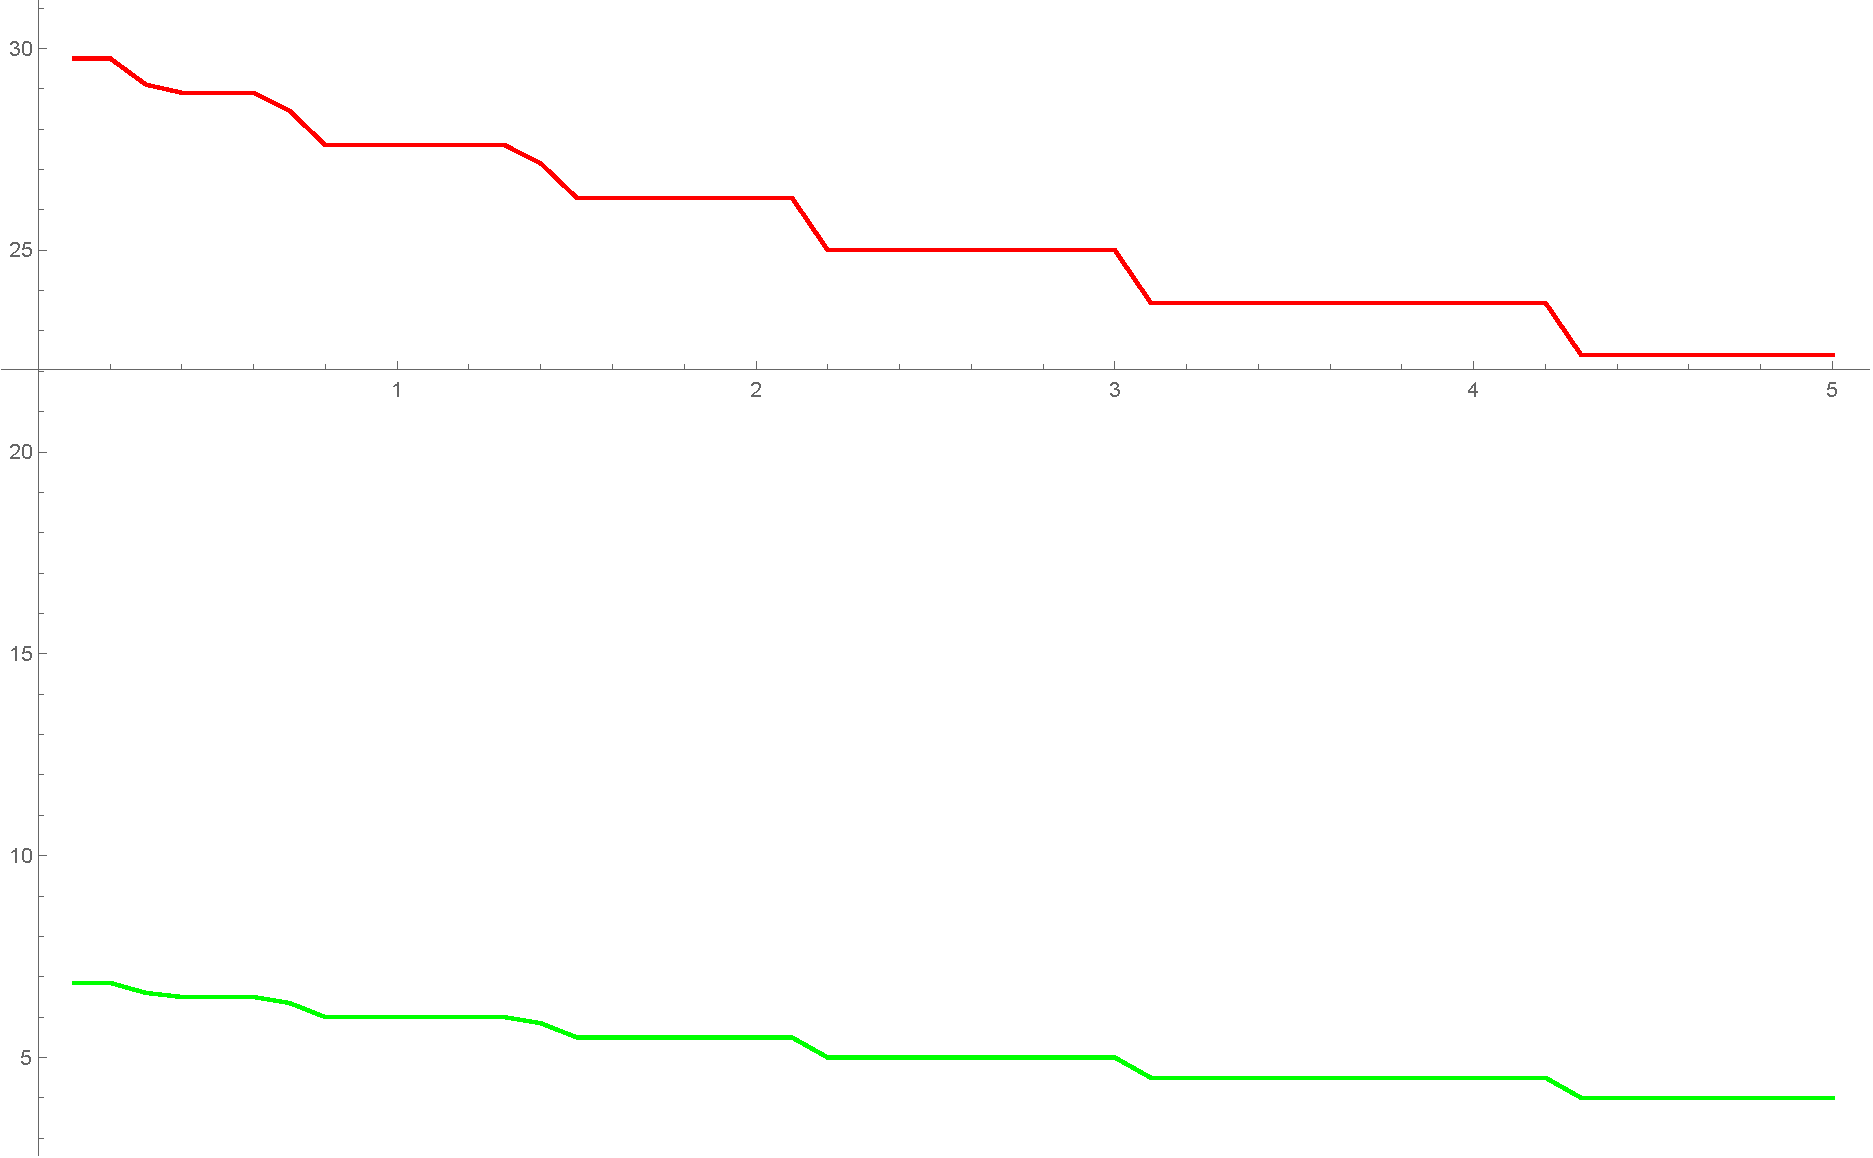
\includegraphics[width=0.8\textwidth]{graf.pdf}
\end{figure}


\end{document}